\chapter{Opis implementacji}
\label{cha:implementacja}

{\it

Zgodnie z założeniami architektury dla proponowanych rozwiązań i przy wykorzystaniu technologii opisanych w poprzednich rozdziałach niniejszej pracy zaimplementowano przykładowe aplikacje prezentujące wykorzystanie koncepcji systemów zarządzania tożsamościami przy użyciu specyfikacji SAML. Najbardziej podstawowym spośród zrealizowanych scenariuszy było zastosowanie asercji SAML w procesie uwierzytelniania klientów aplikacji webowych - udostępnianych poprzez przeglądarkę internetową. Główną rolę w proponowanym rozwiązaniu odgrywa moduł ,,Identity Provider'' odpowiedzialny za procesy uwierzytelniania użytkowników aplikacji.

Implementacja mechanizmów jednokrotnego uwierzytelniania klientów aplikacji webowych przy użyciu standardu SAML była punktem wyjścia dla wdrożenia koncepcji zarządzania tożsamościami dla systemów w architekturze zorientowanej na usługi. Opracowane zostały aplikacje wykorzystujące standard SAML w procesie uwierzytelniania klientów usług webowych(przy użyciu standardów SOAP i REST). Realizacja tych mechanizmów wykorzystuje model architektury uwierzytelniania klientów serwisów webowych opisany w niniejszej  pracy. Zaimplementowano usługi realizujące poszczególne etapy procesu dokonywania zamówienia w sklepie internetowym. Usługi zostały wykorzystane jako przykład zastosowania mechanizmów SAML w architekturze SOA. Wprowadzona została warstwa pośrednicząca pomiędzy wywołaniami klienta a dostarczanymi serwisami - magistrala usług ESB. Zastosowano również narzędzia modelowania procesów biznesowych w celu skomponowania procesu realizacji zamówienia przy użyciu dostępnych usług z wykorzystaniem uwierzytelniania opartego o tokeny bezpieczeństwa SAML. 

}

%---------------------------------------------------------------------------

\autsection{Implementacja mechanizmu jednokrotnego uwierzytelniania klientów aplikacji webowych}{Krzysztof Wilaszek}

	Przy pomocy mechanizmów udostępnianych przez narzędzia \textit{Picketlink} zaimplementowana została usługa ,,Identity Provider'' odpowiedzialna za uwierzytelnianie użytkowników systemu. Stosując usługę IDP możliwe jest jednokrotne uwierzytelnianie klientów aplikacji webowych. Zaimplementowane zostały również aplikacje wykorzystujące usługę IDP jako mechanizm uwierzytelniania klientów żądających dostępu do zasobów aplikacji.

	\begin{figure}[h]
		\centering
		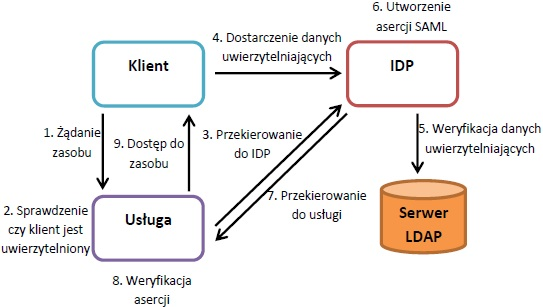
\includegraphics{img/samlWebSSO.jpg}
		\caption{Przebieg procesu jednokrotne uwierzytelnianie aplikacji webowych w protokole SAML}
		\label{samlSSOSteps}
	\end{figure}
		
	Kiedy użytkownik chce uzyskać dostęp do zasobów, usługa sprawdza czy klient jest uwierzytelniony. Jeśli nie jest uwierzytelniony następuje przekierowanie do usługi ,,Identity Provider''. Klient podaje swoje dane uwierzytelniające a IDP weryfikuje ich poprawność. Gdy dane są prawidłowe generowana jest asercja SAML i następuje przekierowanie do usługi. Usługa weryfikuje otrzymaną asercję i przydziela lub odmawia prawa dostępu do zasobu. Gdy klient chce uzyskać dostęp do zasobów innej aplikacji nie musi ponownie podawać swoich danych uwierzytelniających, usługa IDP nie dokonuje ponownie procesu uwierzytelniania w usłudze katalogowej LDAP.
	
	W oparciu o przedstawiony schemat zaimplementowane zostały przykładowe usługi dostarczające funkcjonalności poszczególnych etapów realizacji zamówienia w sklepie internetowym. Opracowano serwisy umożliwiające sprawdzanie stanu magazynu, zlecenie dostawy, obsługę wydawania towarów oraz rejestrację transakcji w serwisie finansowym. Zaimplementowane usługi wykorzystują różne standardy dostarczania usług sieciowych - REST lub SOAP. 

%---------------------------------------------------------------------------

\autsection{Implementacja mechanizmu uwierzytelniania klientów usług webowych}{Krzysztof Wilaszek}

	Implementacja mechanizmów uwierzytelniania klientów usług sieciowych oparta jest na modelu systemu prezentowanym w rozdziale opisującym architekturę dla proponowanych rozwiązań. Zaimplementowane zostały usługi różnych standardów(SOAP i REST) wykorzystujące asercje SAML w procesie uwierzytelniania swoich klientów. Zgodnie z zaproponowanym modelem w systemie istnieje usługa ,,Security Token Service'' odpowiedzialna za przydzielanie tokenów bezpieczeństwa użytkownikom. Otrzymany token bezpieczeństwa dołączany jest do żądania przesyłanego do serwisu. Przed przyznaniem dostępu do żądanych funkcjonalności treść wiadomości przechwytywana jest przez mechanizm specyficzny dla danego typu serwisu. Dla usług opartych o standard SOAP są to mechanizmy typu \textit{,,Handler''}. Dla usług dostarczanych w standardzie REST jest to mechanizm typu \textit{,,Interceptor''} dostarczany przez bibliotekę RESTEasy - implementację technologi dostarczania usług sieciowych typu REST. Mechanizmy dostarczane przez RESTEasy grupują \textit{interceptory} na klasy o różnych priorytetach. Klasą o najwyższym priorytecie(której metody wykonywane są najwcześniej) są \textit{interceptory} bezpieczeństwa. Dzięki zastosowaniu tej grupy możliwa jest realizacja wymagania przeprowadzenia procesu uwierzytelniania klienta na samym początku przetwarzania jego żądania i uniemożliwienia dostępu do jakichkolwiek zasobów dla nieuwierzytelnionych użytkowników.

	\begin{figure}[h]
		\centering
		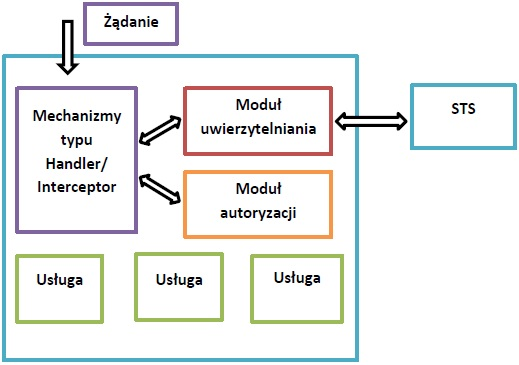
\includegraphics{img/interceptorGatewayImplementation.jpg}
		\caption{Uwierzytelnianie klientów usług webowych przy użyciu asercji SAML}
		\label{interceptorGatewayImplementation}
	\end{figure}

	Przechwycona wiadomość poddawana jest procesom wstępnej analizy. Między innymi wydobywana jest asercja SAML i przy jej wykorzystaniu wykonywany jest proces uwierzytelniania użytkownika. W trakcie uwierzytelniania asercja przesyłana jest do usługi "Security Token Service" w celu weryfikacji jej poprawności. Po poprawnym uwierzytelnieniu klienta usługi następuje proces autoryzacji - dostęp do zasobów przyznawany jest na podstawie wiadomości o przynależności do określonych grup użytkowników. Wiadomość o grupach klienta zawarta jest w asercji SAML.

	W oparciu o przedstawiony schemat zaimplementowane zostały przykładowe usługi dostarczające funkcjonalności poszczególnych etapów realizacji zamówienia w sklepie internetowym. Opracowano serwisy umożliwiające sprawdzanie stanu magazynu, zlecenie dostawy, obsługę wydawania towarów oraz rejestrację transakcji w serwisie finansowym. Zaimplementowane usługi wykorzystują różne standardy dostarczania usług sieciowych - REST lub SOAP. 
	

%---------------------------------------------------------------------------

\autsection{Implementacja mechanizmów bezpieczeństwa w architekturze zorientowanej na usługi}{Krzysztof Wilaszek}

\subsection{Implementacja modułu magistrali usług}

	Implementacja mechanizmu magistrali usług wykorzystuje framework ,,Switchyard''. Przy pomocy narzędzi ,,Switchyard'' konfigurowane są punkty końcowe, na których nasłuchiwane są nadchodzące komunikaty. Przetwarzanie otrzymanych wiadomości realizowane jest przy użyciu narzędzi ,,Camel''. ,,Camel'' dostarcza mechanizmy zarządzania ścieżką jaką kierowane są wiadomości oraz implementuje wzorce EIP(\textit{Enterprise Integration Patterns}). Implementacja mechanizmu przetwarzania wiadomości magistrali usług przedstawiona zostanie na przykładzie wywołań serwisów webowych dostarczanych przy użyciu technologii SOAP(rysunek \textit{,,Implementacja przetwarzania wiadomości przez magistralę usług''}).

	\begin{figure}[h]
		\centering
		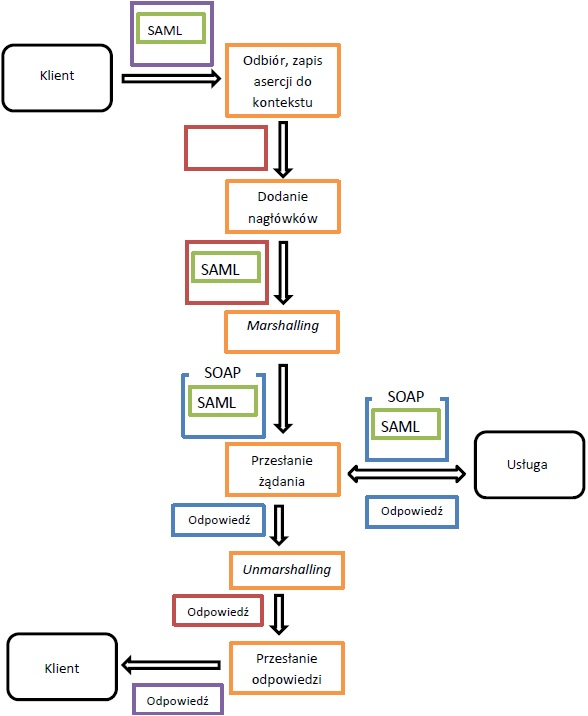
\includegraphics{img/esbRoute.jpg}
		\caption{Implementacja przetwarzania wiadomości przez magistralę usług}
		\label{ESB route}
	\end{figure}

	Klient wywołując usługi przesyła komunikaty określonego formatu - korzystając z określonej metody dostępu do zdalnych serwisów. Moduł magistrali usług otrzymuje komunikat żądania usługi. Do komunikatu dołączony jest nagłówek, w którym przesyłany jest token bezpieczeństwa - asercja SAML. Otrzymany komunikat przekształcany jest do formatu wykorzystywanego wewnętrznie przez moduł przetwarzania wiadomości a informacje zawarte w nagłówku(w tym asercja SAML) zapisywane są w kontekście przetwarzania. Do budowanej wiadomości dodawane są nagłówki(informacje kontekstowe) - dzięki czemu dołączany jest token bezpieczeństwa. Następnie dokonywany jest proces \textit{marshallowania} zbudowanej wiadomości - asercja SAML wpisywana jest do nagłówka(np. SOAP) utworzonego komunikatu. Po serializacji informacji następuje wywołanie usługi korzystające ze zbudowanej wiadomości. Usługa przeprowadza procesy uwierzytelniania klienta i autoryzacji dostępu do zasobów. Po poprawnym przebiegu tych kroków zwracana jest odpowiedź serwisu. Odpowiedź jest \textit{unmarshallowana} i przysłana do klienta w formacie zgodnym z metodą wywołania usługi.

	Dostęp do serwisów obsługujących poszczególne etapy realizacji zamówienia w przykładowym systemie sklepu internetowego odbywa się za pośrednictwem mechanizmu magistrali usług zaimplementowanego zgodnie z opisanym schematem. 
	
	\subsection{Zastosowanie narzędzi modelowania procesów biznesowych}

	Serwisy udostępniane poprzez moduł magistrali usług dostarczają funkcjonalności realizujących poszczególne etapy przetwarzania zamówienia w sklepie internetowym. Przy użyciu narzędzi  zarządzania procesami biznesowymi \textit{jBPM} opracowany został model procesu biznesowego wykorzystujący usługi udostępnianie poprzez moduł magistrali \textit{ESB} w celu realizacji zamówienia w sklepie internetowym. Model zakłada zastosowanie mechanizmów jednokrotnego uwierzytelniania z użyciem standardu \textit{SAML} w procesie uzyskiwania dostępu do usług poszczególnych serwisów realizujących kolejne etapy zamówienia. 

		\begin{figure}[h]
			\centering
			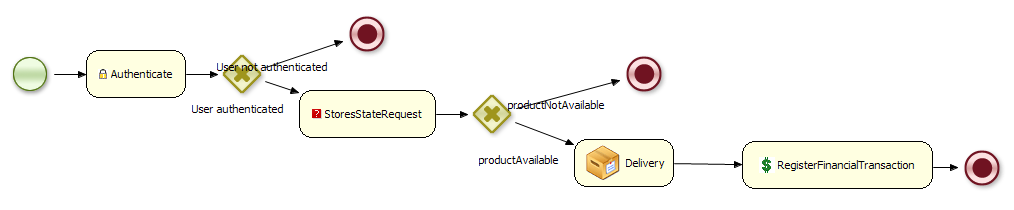
\includegraphics{img/jbpm_order_process.png}
			\caption{Zastosowanie narzędzi modelowania procesów biznesowych z wykorzystaniem mechanizmów jednokrotnego uwierzytelniania}
			\label{jBPM process}
		\end{figure}

	Punktem wejściowym przedstawionego modelu procesu biznesowego jest uwierzytelnienie klienta serwisu. W wyniku poprawnego przebiegu uwierzytelniania klient otrzymuje token bezpieczeństwa - asercję SAML. Uzyskana asercja wykorzystywana jest w procesie przyznawania dostępu do usług konkretnych serwisów odpowiadających za poszczególne etapy realizacji zamówienia. Zastosowanie asercji SAML i wykorzystanie modelu opisanego przez specyfikację WS-Trust pozwala na osiągnięcie funkcjonalności jednokrotnego uwierzytelniania klienta procesu biznesowego - token bezpieczeństwa pozyskany na etapie uwierzytelniania identyfikuje klienta aplikacji podczas korzystania z usług poszczególnych serwisów wchodzących w skład procesu.
%---------------------------------------------------------------------------
